
\Chapter{Joint Intrinsic Motivation}{Inducing coordinated exploration in multi-agent environments.}

\label{ChapterJIM} 

\textit{This chapter extends the conference paper "}Joint Intrinsic Motivation for Coordinated Exploration in Multi-Agent Deep Reinforcement Learning\textit{", published in the Conference on Autonomous Agents and Multi-Agent Systems (AAMAS) 2024\footnote{Full paper available at: \url{https://arxiv.org/abs/2402.03972}}.}

% \vspace{4em}

\section{Introduction}


In Chapter~\ref{ChapterMADRL}, we reviewed the multi-agent deep reinforcement learning (MADRL) literature, its state-of-the-art approaches, and some important challenges that still need to be tackled for building better learning algorithms. 
One major issue in multi-agent learning is the problem of relative overgeneralisation~\citep{Wiegand2003_RelOvergen, Wei2016_RelOvergen} where agents struggle to find the optimal joint policy because local policies are attracted towards suboptimal areas of the search space. This makes most algorithms inefficient in tasks where the optimal strategy requires strong coordination among agents. Relative overgeneralisation can be described as a problem of exploration of the joint-observation space: as the success of the MAS depends on the coordination of multiple agents, exploring the joint-observation space is required to discover optimal joint behaviours. In this chapter, we address the question of how to explore the joint-state space to efficiently discover superior coordinated strategies for solving the task at hand. 

In single-agent RL, the problem of exploration has been studied to solve hard exploration tasks where positive reward signals are sparse. One solution is to use intrinsic motivation~\citep{Schmidhuber1991, Oudeyer2007_IntrMotiv, lehman2011abandoning} to incite agents to explore unknown parts of the environment. In addition to the environment reward, agents are given an auxiliary reward related to the novelty of encountered states. Maximising this intrinsic reward leads agents to visit previously unexplored regions of the environment, ultimately discovering new solutions to the task. These methods have shown great success in helping RL agents solve hard exploration tasks \citep{Pathak2017_ICM, Badia2020_NGU}. 

In the multi-agent setting, intrinsic objectives have also been studied to induce different kinds of behaviours in agents such as coordinated exploration \citep{Iqbal2019_MultiExplore}, social influence \citep{Jaques2019_SocialInfluence, Wang2020_EITI} or alignment with other agents' expectations \citep{Ma2022_ELIGN}. However, previous works have only used local observations to generate intrinsic rewards. With partial observability, local observations often lack crucial information to fully understand the current configuration of the environment. In the context of exploration, an intrinsic reward based only on local observations will lead to each agent exploring their own observation space, without considering the current state of other agents. This can result in inefficient exploration in cooperative tasks where the success of the MAS depends on the coordination of all agents.

In this chapter, we introduce a novel multi-agent exploration approach called \textbf{Joint Intrinsic Motivation} (JIM) which can be combined with any MADRL algorithm that follows the centralised training with decentralised execution (CTDE) para\-digm. JIM exploits centralised information during training to motivate agents to explore new coordinated behaviours. In order to compute joint novelty, JIM builds from two state-of-the-art single-agent intrinsic rewards: NovelD \citep{Zhang2021_NovelD} for exploring unknown parts of the environment, and E3B \citep{Henaff2022_E3B} for having more diverse trajectories. Adding this auxiliary reward to the agents' objective incites them to diversify their collective behaviour until they have a fair knowledge of the environment and can focus on the main task at hand. 

To demonstrate the advantages of our approach, we first design a simple test environment to showcase a clear example of relative overgeneralisation. We show that the state-of-the-art algorithm QMIX \citep{Rashid2018_QMIX} struggles in this scenario and that motivating the exploration of coordinated behaviour helps solve the task. Next, we validate these results in a continuous virtual environment, showing that coordination tasks benefit from joint exploration. Finally, further analysis is conducted to confirm the strength and scalability of our approach.






% -------------------------------------------------------------------------------------------------

\section{The Multi-Agent Exploration Problem}\label{sec:JIM:ExploProblem}

\subsection{Random Exploration Strategies}

% Random exploration strategies
To effectively learn with RL, algorithms need to balance an exploration-exploitation trade-off. Exploration of the environment is required to collect knowledge about the task. But, exploiting the learnt strategy allows focusing on parts of the environment that were discovered valuable, potentially making learning more efficient. 
Most RL methods tackle this issue by adding randomness in the agents' behaviour during training. Algorithms based on Q-learning use the $\epsilon$-greedy strategy, described in Section~\ref{sec:RL:Qlearning}, where agents start training by executing random actions and progressively shift to choosing actions only using the learnt action-value. 
In policy-based approaches, multiple exploration strategies are possible. 
In DDPG~\citep{Lillicrap2015_DDPG} and the multi-agent version MADDPG~\citep{Lowe2017_MADDPG}, exploration is performed by adding a Gaussian noise on the action generated by the deterministic formula: $a^i_t=\pi_i(o^i_t)+\epsilon$, with the noise $\epsilon\sim\mathcal{N}(0,\sigma)$ and $\sigma$ a hyperparameter controlling the standard variation of the exploration noise. 
In PPO~\citep{Schulman2017_PPO} and MAPPO~\citep{Yu2021_MAPPO}, because the policy is stochastic, actions can be drawn randomly from the generated action distribution during training: $a^i_t\sim\pi(.|o^i_t)$. In addition to this, exploration is also handled at the policy learning level, by maximising the entropy of the policy in the PPO objective (see Equation~\ref{eq:PPO-objective}). 
% (? Note that, because policies are independent in MADDPG and MAPPO, this means that exploration is done locally, which may induce non-stationarity?)

% Hard exploration problem in single-agent RL
All these approaches rely on randomness to ensure that agents gather essential knowledge about the environment and the task. However, in environments with very few positive reward signals, random exploration is not sufficient~\citep{Ostrovski2017_PseudoCounts, Pathak2017_ICM, Burda2019_RND}. In hard exploration problems, finding the positive reward signal requires specific sequences of hundreds of actions with no guidance. Discovering these trajectories by acting randomly is extremely unlikely. And, to be able to learn an efficient behaviour, RL algorithms require experiencing this behaviour many times, learning a little bit from each experience. Thus, random exploration is unlikely to enable efficient discovery and learning of optimal strategies in hard exploration problems. 





\subsection{Relative Overgeneralisation}\label{sec:JIM:RelOvergen}

% Relative overgeneralisation
\begin{figure}[t]
    \centering
    \begin{tabular}{c|c|c|c|}
        \multicolumn{1}{c}{} & \multicolumn{1}{c}{$A$}  & \multicolumn{1}{c}{$B$}  & \multicolumn{1}{c}{$C$} \\\cline{2-4}
        $A$ & $10$ & $-5$ & $-5$ \\\cline{2-4}
        $B$ & $-5$ & $7$ & $7$ \\\cline{2-4}
        $C$ & $-5$ & $7$ & $7$ \\\cline{2-4}
    \end{tabular}
    % \subcaptionbox{\label{fig:JIM:ro_map}}{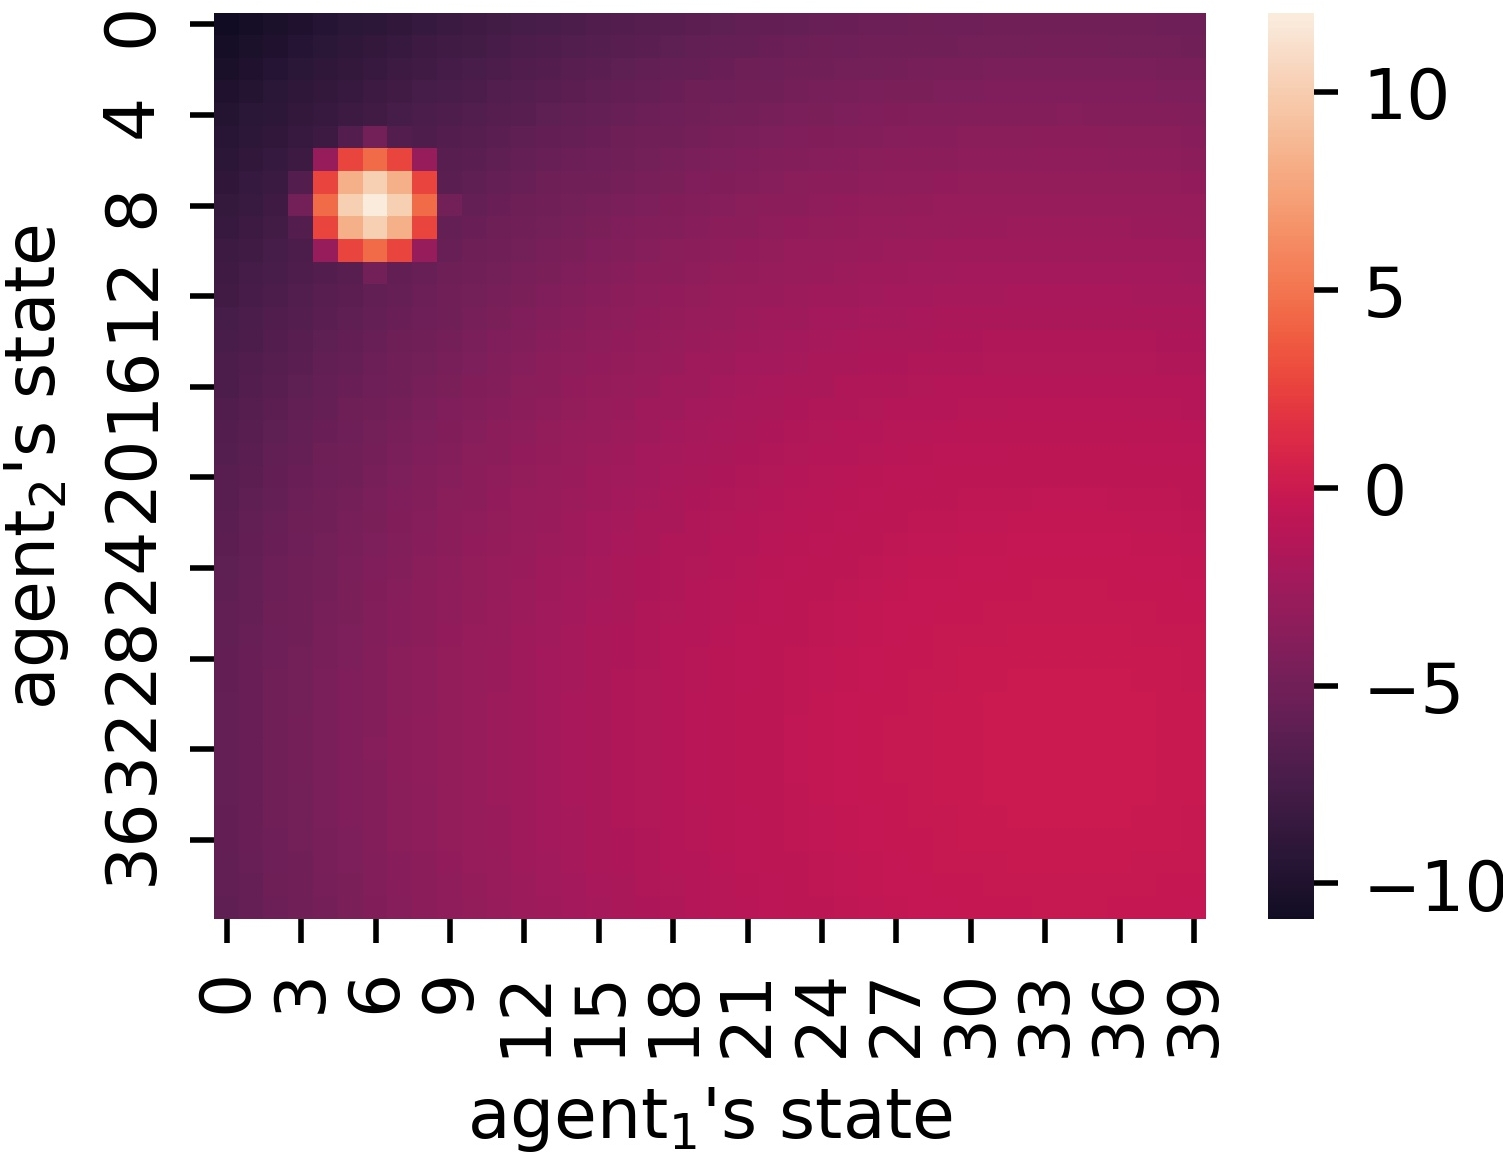
\includegraphics[width=0.45\textwidth]{Figures/JIM/ro_map30.jpg}}
    \caption{A social dilemma featuring the problem of relative overgeneralisation. Two agents have to choose between three actions. The optimal joint behaviour is both agents choosing action A. But, because actions B and C have a better average return when looked at locally, they will often be preferred.}
    \label{fig:JIM:ro_matrix}
\end{figure}

% Coordination is hard-exploration
The hard exploration problem becomes even worse in MAS as the completion of a task depends on the actions of multiple independent agents. In the context of MAS, a task that requires strong coordination between multiple agents can be considered a hard exploration problem. As defined in Section~\ref{sec:MAL:Coordination}, coordination requires the synchronisation of multiple agents' actions to achieve their common goal. Thus, a task requiring strong coordination is one where very few joint behaviours will produce the optimal returns. As in single-agent hard exploration problems, consistently discovering these optimal joint trajectories through random exploration will be extremely inefficient. 

In such cases, agents learning by randomly exploring their local state-action spaces will often struggle to find the optimal coordination strategy and settle for an easier suboptimal joint strategy. This is a problem known as \textbf{relative overgeneralisation}~\citep{Wiegand2003_RelOvergen, Wei2016_RelOvergen}, illustrated in Figure \ref{fig:JIM:ro_matrix}. In this example, there are two Nash equilibria: the optimal equilibrium with both agents choosing action A, and a suboptimal equilibrium where agents choose randomly between actions B and C with any probability. While the joint action (A, A) is clearly optimal, if agents explore their actions locally they will quickly find that actions B and C yield better returns on average. Only if all joint actions are explored and evaluated against each other, will the agents discover the optimal joint strategy. Thus, a joint-exploration approach can help solve the issue of relative overgeneralisation.







% -------------------------------------------------------------------------------------------------

\section{Explicit Exploration Strategies: Related Works}\label{sec:JIM:RelatedWorks}

% Faire une sous section pour :
% Exploration and Intrinsic rewards in single agent RL (parler de GoExplore, NGU, Agent57)
% Méthodes d'exploration multi plus poussées (hysteretic, leniency, MAVEN...)
% Intrinsic rewards in maRL

\subsection{Exploration in Single-Agent Reinforcement Learning}

To improve the exploration strategies of RL agents, multiple techniques have been employed. Inducing noise in learnt estimates can help RL agents having more diverse behaviour during training~\citep{Osband2016_BootstrappedDQN, Fortunato2018_NoisyDQN, Plappert2018_Noise, Osband2018_RandomizedValue, Chiappa2023_Lattice}. Hierarchical learning algorithms can be driven by the search for new skills, based on the idea that different skills generate different trajectories~\citep{Gregor2017_VIC, Eysenbach2019_DIAYN, Gehring2021_HierarchicalSkills}. Other works use a learnt model of the environment to plan exploration trajectories~\citep{Shyam2019_MAX, Sekar2020_Plan2Explore, Hu2023_PlanGoalExplore}. \cite{Ecoffet2021_GoExplore} achieve great results on hard exploration problems with a more handcrafted exploration method based on replaying past trajectories that resulted in unknown states, and starting exploring randomly from these states. Similarly, \cite{Pislar2022_WhenExplore} devise a strategy to decide when agents should explore with random actions based on their knowledge of the environment. 

However, the most successful approach for solving hard exploration problems has been inciting curiosity with intrinsic motivation. 
\textbf{Intrinsic motivation} is a technique for shaping the behaviour of RL agents by adding an auxiliary reward for them to maximise~\citep{Schmidhuber1991, Oudeyer2007_IntrMotiv, lehman2011abandoning}. This reward is computed by the agent, hence the name "intrinsic reward", based on its current state. Curiosity can be induced by computing a reward based on the novelty of the agent's trajectory. By learning to maximise this curiosity objective, the agent should learn to search for novel states. 
% In single-agent RL, curiosity has been defined to help agents solve hard exploration tasks~\citep{Schmidhuber1991,Oudeyer2007_IntrMotiv,lehman2011abandoning} by rewarding the visitation of states considered as novel. 
For measuring novelty, several methods use the error of trainable prediction models. The \textit{Intrinsic Curiosity Module} (ICM) \citep{Pathak2017_ICM} trains a model of environment dynamics and uses the prediction error as a measure of novelty. \textit{Random Network Distillation} (RND) \citep{Burda2019_RND} uses a neural network with fixed, randomly initialised parameters to produce a random encoding of the state, and trains a predictor network to generate the same encoding, the prediction error being the measure of novelty. With these two approaches, the prediction models will yield low novelty for states similar to what they have trained on, while producing high novelty for unknown parts of the environment. RIDE \citep{Raileanu2020_RIDE} and NovelD \citep{Zhang2021_NovelD} use respectively ICM and RND to compute a reward from the difference of novelty between the next state and the current state, pushing the agents to always seek novel states. Similarly, NGU \citep{Badia2020_NGU} and E3B \citep{Henaff2022_E3B} use clustering techniques to reward states that are distant from previously observed states. Agent57~\citep{Badia2020_Agent57} manages to solve the hard exploration games in the Atari benchmark by extending NGU to learn two value functions: one for the extrinsic reward and one for the intrinsic one; and by learning a meta-controller that decides whether to explore or exploit during training. Finally, AGAC \citep{FletBerliac2021_AGAC} trains an adversarial policy to predict the main policy’s output, the latter being rewarded with the former’s prediction error. 
%In our case, we choose to combine NovelD and E3B for their performance and simplicity.



\subsection{Exploration in Multi-Agent Reinforcement Learning}

% Leniency, hysteretic, MAVEN

To address the problem of relative overgeneralisation, better exploration strategies must be implemented in MADRL algorithms. Not all single-agent exploration strategies can be used efficiently in multi-agent settings. The noise-inducing approach could be another source of non-stationarity in a multi-agent algorithm. Also, plan\-ning-based techniques are not usable as learning a model in a multi-agent setting is challenging. However, some other approaches have been successfully pursued. 
MAVEN \citep{Mahajan2019_MAVEN} extends QMIX with a hierarchical policy that chooses goals common to all agents, and then explores the space of these joint goals to try different joint behaviours. 
Similarly, CMAE~\citep{Liu2021_CMAE} have agents sharing common goals, defined as states to reach, and use a curriculum approach for choosing joint goals of increased difficulty based on the number of times each goal-state has been experienced. 
\cite{Lupu2021_TrajeDi} promote policy diversity by learning a population of agents and maximising the divergence of each policy with regards to the rest of the population, which is shown to help agents be more versatile. 
Finally, EMAX~\citep{Schafer2023_EMAX} learn multiple joint value functions at once and explore by maximising the disagreement of the ensemble of joint values. 
% MAVEN 
% MultiSoftQ maximise the entropy of local policies in a MADDPG-style architecture
% Liu2021_CMAE learns to achieve subgoals that are gradually more diverse
% Schafer2023_EMAX learn an ensemble of joint value functions and drive exploration by rewarding agent locally with the disagreement of the ensemble of value

\subsection{Multi-Agent Intrinsic Motivation}

In MASs, there is a large variety of different ways to complete tasks, interact with teammates, and handle opponents. Different definitions of intrinsic motivation can stimulate the emergence of different types of behaviour. 
Social influence has been shown to help learn interesting multi-agent behaviour~\citep{Jaques2019_SocialInfluence, Wang2020_EITI}, by rewarding actions that have a significant impact on other agents. Learning to influence other agents helps train agents that actively look for interactions, thus avoiding lazy agents, and that try new behaviours during training, helping the exploration of joint behaviours. \cite{Ma2022_ELIGN} propose an intrinsic reward based on the average alignment with other agents' expectations. Depending on how this alignment reward is used, as a bonus or a penalty, this can promote more predictable or more surprising behaviours. 

Curiosity has also been studied for multi-agent exploration. ~\cite{Iqbal2019_MultiExplore} propose an approach for coordinated exploration using several metrics for estimating the novelty of observations that depend on all agents' past experiences. \cite{Zheng2021_EMC} extend VDN with a separate network that predicts local action-values, with an intrinsic curiosity reward based on the prediction error of these separate values. Finally, in a concurrent work, COIN~\citep{Li2023_COIN} proposed an intrinsic reward inspired by ICM that measures the novelty of the joint trajectories. Apart from COIN, other multi-agent intrinsic rewards use local observations for computing their intrinsic rewards. As shown in Section~\ref{sec:JIM:RelOvergen}, local exploration is not sufficient for exploring coordinated behaviours. Therefore, in the following sections, we present an approach for exploring the space of joint observations with an intrinsic reward inspired by recent works in single-agent curiosity. 








% -------------------------------------------------------------------------------------------------

\section{Background on Intrinsic Reward Definitions}\label{sec:JIM:IntrRew}


% Faire de chaque paragraph une sous section et étendre un peu si possible?


In Section \ref{sec:JIM:RelatedWorks}, we introduced intrinsic motivation as a way to incite agents to actively explore their environment. To this end, at each time step $t$, agents receive an augmented reward $r_t=r^{\text{ext}}_t+\beta r^{\text{int}}_t$, where $r^{\text{ext}}_t$ is the extrinsic reward given by the environment, $r^{\text{int}}_t$ is the intrinsic reward, and $\beta$ is a hyperparameter controlling the weight of the intrinsic reward in the agents' objective. We describe three methods of intrinsic motivation from the literature that we will use later in Section~\ref{sec:JIM:Algo}. 




\subsection{Random Network Distillation (RND)}\label{sec:JIM:RND}

In \textit{random network distillation} (RND), \cite{Burda2019_RND} compute novelty using two neural networks with the same architecture: a target network $\phi$ and a predictor network $\phi'$. The target's parameters are initialised randomly and fixed. It takes as input the state $s_t$ and produces a random embedding $\phi(s_t)$. The predictor is trained to output the same embedding, minimising the Euclidean distance:
\begin{equation}\label{eq:JIM:RND}
    RND(s_t)=\lVert\phi(s_t)-\phi'(s_t)\rVert_2.
\end{equation}
By training the predictor network to produce the same embeddings as the one generated by the target, the algorithm essentially tries to copy the parameters of the target in the predictor, or "distil" them. This distance $RND(s_t)$ is also used as a measure of the novelty of state $s_t$ and is given as an intrinsic reward to the agent. By training the predictor network along the agent, the predictor will get better at predicting the embeddings of states that are often seen by the agent during its trials. Thus, to accumulate more intrinsic reward, the agent will have to discover new states. 




\subsection{Novelty Diversity (NovelD)} \label{sec:JIM:NovelD}

Zhang et al.~\citep{Zhang2021_NovelD} build upon RND to devise a novelty criterion termed \textit{NovelD}, for "novelty diversity". It is defined as follows:
\begin{equation}\label{eq:JIM:NovelD}
    N(s_t, s_{t+1}) = \mathrm{max}[RND(s_{t+1}) - \alpha RND(s_t), 0]\times\mathds{1}\{N_e(s_{t+1})=1\},
\end{equation}
with $\alpha$ a scaling factor, $N_e$ an episodic count of visited states, and $\mathds{1}\{\cdot\}$ the indicator function that outputs $1$ if the condition is true. The first part is the core of the novelty criterion. It uses RND to reward agents for positive gains in novelty between the current and the next states. Thus, NovelD rewards the agent for always going towards newer states. The second part is an episodic restriction that ensures the reward is given only when state $s_{t+1}$ is observed for the first time in this episode. This ensures that agents cannot exploit one particularly novel state by staying in it. However, because this restriction is based on an explicit count of the occurrence of states during the episode, it limits the use of NovelD to discrete state spaces, as continuous states will likely never be reached more than once. 



\subsection{Exploration via Elliptical Episodic Bonuses (E3B)}\label{sec:JIM:E3B}

\cite{Henaff2022_E3B} propose \textit{exploration via elliptical episodic bonuses} (E3B), an episodic bonus based on the position of the observed state with respect to an ellipse that fits all states previously encountered in the current episode. Formally, it is computed as follows:
\begin{equation}\label{eq:JIM:E3B}
    b(s_t)=\psi(s_t)^\top C^{-1}_{t-1}\psi(s_t),
\end{equation}
with
\begin{equation}
    C_{t-1}=\sum_{i=1}^{t-1}\psi(s_i)\psi(s_i)^\top+\lambda I,
\end{equation}
where $I$ is the identity matrix and $\lambda$ a scalar coefficient. $\psi$ is an embedding network trained using an inverse dynamics model \citep{Pathak2017_ICM}: embeddings of following states $\psi(s_t)$ and $\psi(s_{t+1})$ are used by a separate neural network trained to predict the action $a_t$ taken between these states. As a result of this training process, $\psi$ encodes parts of the observation that are controllable by the agents (see the original paper for more detail,~\cite{Henaff2022_E3B}). Intuitively, $b$ can be understood as a generalisation of a count-based episodic bonus for a continuous state space. States that are close to previously encountered states in the current episode will yield low bonuses, whereas states that are very different will produce high bonuses. This incites the agent to have diverse trajectories. 







% -------------------------------------------------------------------------------------------------


\section{Joint Intrinsic Motivation Algorithm}\label{sec:JIM:Algo}

In this section, we introduce the Joint Intrinsic Motivation (JIM) exploration criterion for coordinated multi-agent exploration. We take inspiration from state-of-the-art intrinsic motivation techniques developed for single-agent RL and propose a new method for efficient multi-agent exploration. 
First, we define the main components of the intrinsic reward. Then, we explain how it is used in a multi-agent setting for exploring the space of joint observations. 


\subsection{Double-timescale Intrinsic Reward}\label{sec:JIM:DoubleTimeReward}

Similarly to previous works on single-agent intrinsic motivation~\citep{Badia2020_NGU}, we define a novelty metric that combines two exploration criteria working at different timescales:
\begin{itemize}
    \item A \textbf{life-long exploration criterion (LLEC)} that captures how novel is the current observation with respect to all observations since the beginning of training.
    \item An \textbf{episodic exploration criterion (EEC)} that captures the difference between the current observation and all previous observations in the current episode. 
\end{itemize}
Intuitively, the \textit{life-long reward} motivates agents to search for never-experienced parts of the environment. Meanwhile, the \textit{episodic bonus} induces more diverse trajectories. These two elements will work together to reinforce agents to efficiently explore their environment. 

We first define this intrinsic reward as it would be in a single-agent case, measuring the novelty of an agent's state. For each transition from state $s_t$ to the next state $s_{t+1}$, we define the double-timescale intrinsic reward as follows: 
\begin{equation}\label{eq:JIM:IntrRew}
    r_t(s_t, s_{t+1}) = N_{LLEC}(s_t,s_{t+1})\times N_{EEC}(s_{t+1}),
\end{equation}
with the life-long novelty $N_{LLEC}$ inspired from NovelD~\citep{Zhang2021_NovelD} (see Eq.~\eqref{eq:JIM:NovelD}):
\begin{equation}\label{eq:JIM:LLEC}
    N_{LLEC}(s_t, s_{t+1}) = \mathrm{max}[RND(s_{t+1}) - \alpha RND(s_t), 0],
\end{equation}
with $\alpha$ a scaling factor and $RND$ the novelty measure (see Eq.~\eqref{eq:JIM:RND}). Further, the episodic novelty $N_{EEC}$ uses the bonus from E3B~\citep{Henaff2022_E3B} (see Eq.~\eqref{eq:JIM:E3B}):
\begin{equation}\label{eq:JIM:EEC}
    N_{EEC}(s_{t+1}) = \sqrt{2b(s_{t+1})}.
\end{equation}

We make two modifications compared to previous works. First, we modify NovelD by removing the count-based episodic restriction that was limited to discrete state spaces. We replace it with the elliptical episodic bonus $b$ from E3B~\citep{Henaff2022_E3B}. This bonus acts as an episodic restriction by scaling $N_{LLEC}$ up or down, depending on the novelty of the current state compared to what has been observed during the current episode. Second, we take $\sqrt{2b(s_{t+1})}$ instead of simply $b$ to smooth the values given by this bonus, increasing the small ones and decreasing the large ones. This is because we observed that, in continuous state spaces (which was not studied in the original E3B paper), $b$ yielded extremely high bonuses at the start of the episode and quickly dropped to low bonuses after this. Thus, the smoothing function allows having a more controlled range of bonuses. 

Combining these two rewards makes it possible to take the benefits of both. $N_{LLEC}$ pushes agents to explore regions of the state space that are not well-known to agents, considering states observed since the beginning of training. Meanwhile, $N_{EEC}$ favours diverse trajectories, inciting agents to always seek new observations during a single episode. As the agents explore their environment, the prediction error of RND (see Eq.~\eqref{eq:JIM:RND}) slowly decreases. Thus, $N_{LLEC}$ decreases as well, tending toward zero. This allows to naturally shift from high exploration at the beginning of training, to progressively focusing on the extrinsic reward. Finally, as the episodic restriction does not rely on any explicit count of visited states, it can be used in continuous state spaces. 




\subsection{The Joint Intrinsic Motivation Algorithm}

\begin{figure}[h]
    \centering
    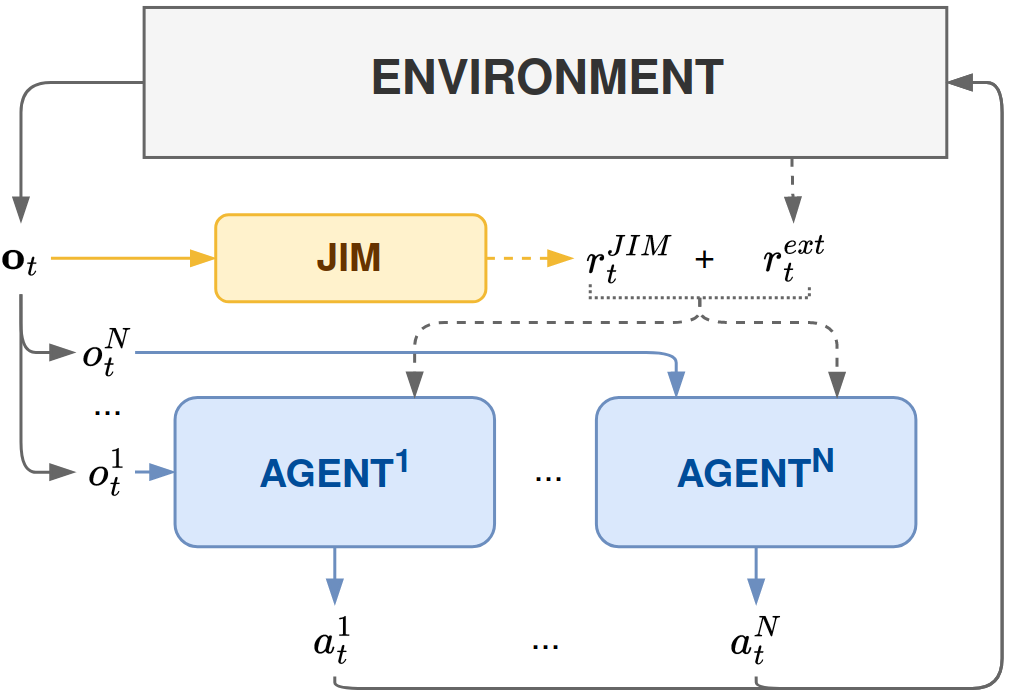
\includegraphics[width=0.6\textwidth]{Figures/JIM/archi_jim.png}
    \caption{Architecture for the Joint Intrinsic Motivation (JIM) algorithm. JIM has only one intrinsic motivation module for the whole multi-agent system, computing novelty of the joint observation $\mathbf{o}_t$. However, agents only use their local observation to choose their actions.}
    \label{fig:JIM:archi}
\end{figure}

Building from the intrinsic reward introduced previously, we propose the \textbf{Joint Intrinsic Motivation} (JIM) algorithm to incite MADRL agents to explore the joint-observation space. At each time step, all agents receive the same global reward $r_t=r^{\text{ext}}_t+\beta r^{JIM}_t$, where $r^{\text{ext}}_t$ is the extrinsic reward given by the environment, $r^{JIM}_t$ is our joint exploration criterion, and $\beta$ is a hyperparameter controlling the weight of the intrinsic reward. The exploration criterion in JIM uses the double-timescale intrinsic reward defined previously to compute the novelty of the joint observation:
\begin{equation}\label{eq:JIM:JIM}
    r_t^{JIM}(\mathbf{o}_t,\mathbf{o}_{t+1})=N_{LLEC}(\mathbf{o}_t,\mathbf{o}_{t+1})\times N_{EEC}(\mathbf{o}_{t+1}),
\end{equation}
where $\mathbf{o}_t=\{o_t^i\}_{0\leq i\leq N}$, i.e., the concatenation of all local observations. Figure \ref{fig:JIM:archi} shows the architecture for JIM. Compared to a local method that would use one intrinsic motivation module per agent, JIM computes only one intrinsic reward. This makes it possible to capture novelty at the team level, rather than at the individual level only, while requiring fewer parameters and less computation. As agents are rewarded by the novelty of the joint observation, they will learn to search for new combinations of observations with other agents of the system, rather than only exploring their local-observation space. This will induce the exploration of new configurations of the environment and thus help find better coordinated strategies.

As JIM uses joint observations for computing the intrinsic reward, it can be associated with any MADRL algorithm that fits in the CTDE paradigm. These algorithms usually employ a centralised value function \citep{Lowe2017_MADDPG,Rashid2018_QMIX,Yu2021_MAPPO} that looks at the joint observation to predict the value of the agents' actions. Such centralised value functions will be able to associate rewards provided by JIM to new configurations in the joint observation space, thus inducing agents to actively search for these configurations. 

One could note that the joint observation has two notable drawbacks: the number of dimensions grows linearly with the number of agents and there is a risk of capturing redundant information. These issues are both alleviated by using embedding networks to encode the joint observation into a more condensed latent representation. Both $N_{LLEC}$ and $N_{EEC}$ use embedding networks, respectively $\phi$ and $\psi$ (as described in Section~\ref{sec:JIM:IntrRew}), to encode the joint observation. This allows for a more controllable number of parameters in JIM, as only the dimension of the input layers of $\phi$ and $\psi$ depend on the size of the joint observation. Furthermore, embedding networks learn to cast away useless or redundant information in order to produce a more compact representation of the joint observation. Note that both $\phi$ and $\psi$ were originally used (respectively in RND \citep{Burda2019_RND} and E3B \citep{Henaff2022_E3B}) with raw pixel images as input, showing the significant capability of dimensionality reduction of these techniques.

%Another option would be to use a global state of the environment comprising all information available in the environment in place of the joint observation. However, not all environments are able to provide such a global state. Thus, we choose not to pursue this idea and stick with the concatenation of all local observations.







% -------------------------------------------------------------------------------------------------

\section{Implementation Details}\label{sec:JIM:ImpDetails}

\begin{figure}[t]
    \centering
    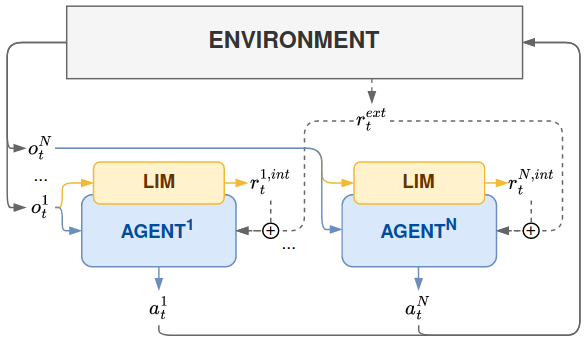
\includegraphics[width=0.71\textwidth]{Figures/JIM/archi_lim.png}
    \caption{Architecture for local intrinsic motivation (LIM), used as a baseline. Each agent has its own module for computing an intrinsic reward based on its local observation.}
    \label{fig:JIM:archi_lim}
\end{figure}

%As previously said, JIM can be used to augment any MADRL approach that fits in the CTDE paradigm. 
In the next section, we use JIM with QMIX~\citep{Rashid2018_QMIX}. We use the default QMIX architecture and hyperparameters, along with prioritised experience replay~\citep{Schaul2016_PER}. In all experiments, we compare three algorithms: 
\begin{itemize}
    \item \textbf{QMIX+JIM}, augmenting QMIX with joint exploration, as shown in Figure~\ref{fig:JIM:archi} and described in Section~\ref{sec:JIM:IntrRew}.
    \item \textbf{QMIX+LIM}, a degraded version of QMIX+JIM where local intrinsic motivation is used. Each agent generates its own intrinsic reward based solely on its local observation, using the same reward definition as JIM (see Section~\ref{sec:JIM:IntrRew}). The architecture for LIM (Local Intrinsic Motivation) is described in Figure~\ref{fig:JIM:archi_lim}.
    \item The original state-of-the-art \textbf{QMIX} algorithm~\citep{Rashid2018_QMIX} with no intrinsic motivation, used as a baseline. 
\end{itemize}
Note that the only difference between these three algorithms is the definition of the reward function given to each agent during training. The actual training and execution algorithms are identical. 

To ensure a fair comparison between JIM and LIM, we use different values for some specific hyperparameters in the two versions in order for them to have a similar number of trainable parameters. All hyperparameters used in our experiments are listed in Appendix~\ref{app:JIM:hpp}. The code used to run all experiments is freely available online\footnote{\url{https://github.com/MToquebiau/Joint-Intrinsic-Motivation}}.







% -------------------------------------------------------------------------------------------------

\section{Experiments}

In this section, we present a set of experiments to evaluate the exploration criterion of JIM when used along the state-of-the-art QMIX algorithm \citep{Rashid2018_QMIX}. First, we show the results in a synthetic discrete environment where the problem of relative overgeneralisation can be artificially tuned and observe that JIM helps alleviate this issue. Then, we test our approach on pseudo-realistic robotic tasks in a continuous environment and show that exploring the joint-observation space helps solve cooperative tasks with strong coordination requirements. Next, we present an ablation study by comparing JIM with two simpler versions that each lack one of the two exploration criteria described in Section~\ref{sec:JIM:IntrRew}, showing the advantage of combining the two. We show that JIM remains efficient with more than two agents. And, finally, we show that the centralised intrinsic motivation is more computationally efficient than the local version. 

\subsection{Addressing Relative Overgeneralisation}
\label{sec:JIM:Exp_Climbing}

\subsubsection{Environment Definition}

\begin{figure}
    \centering
    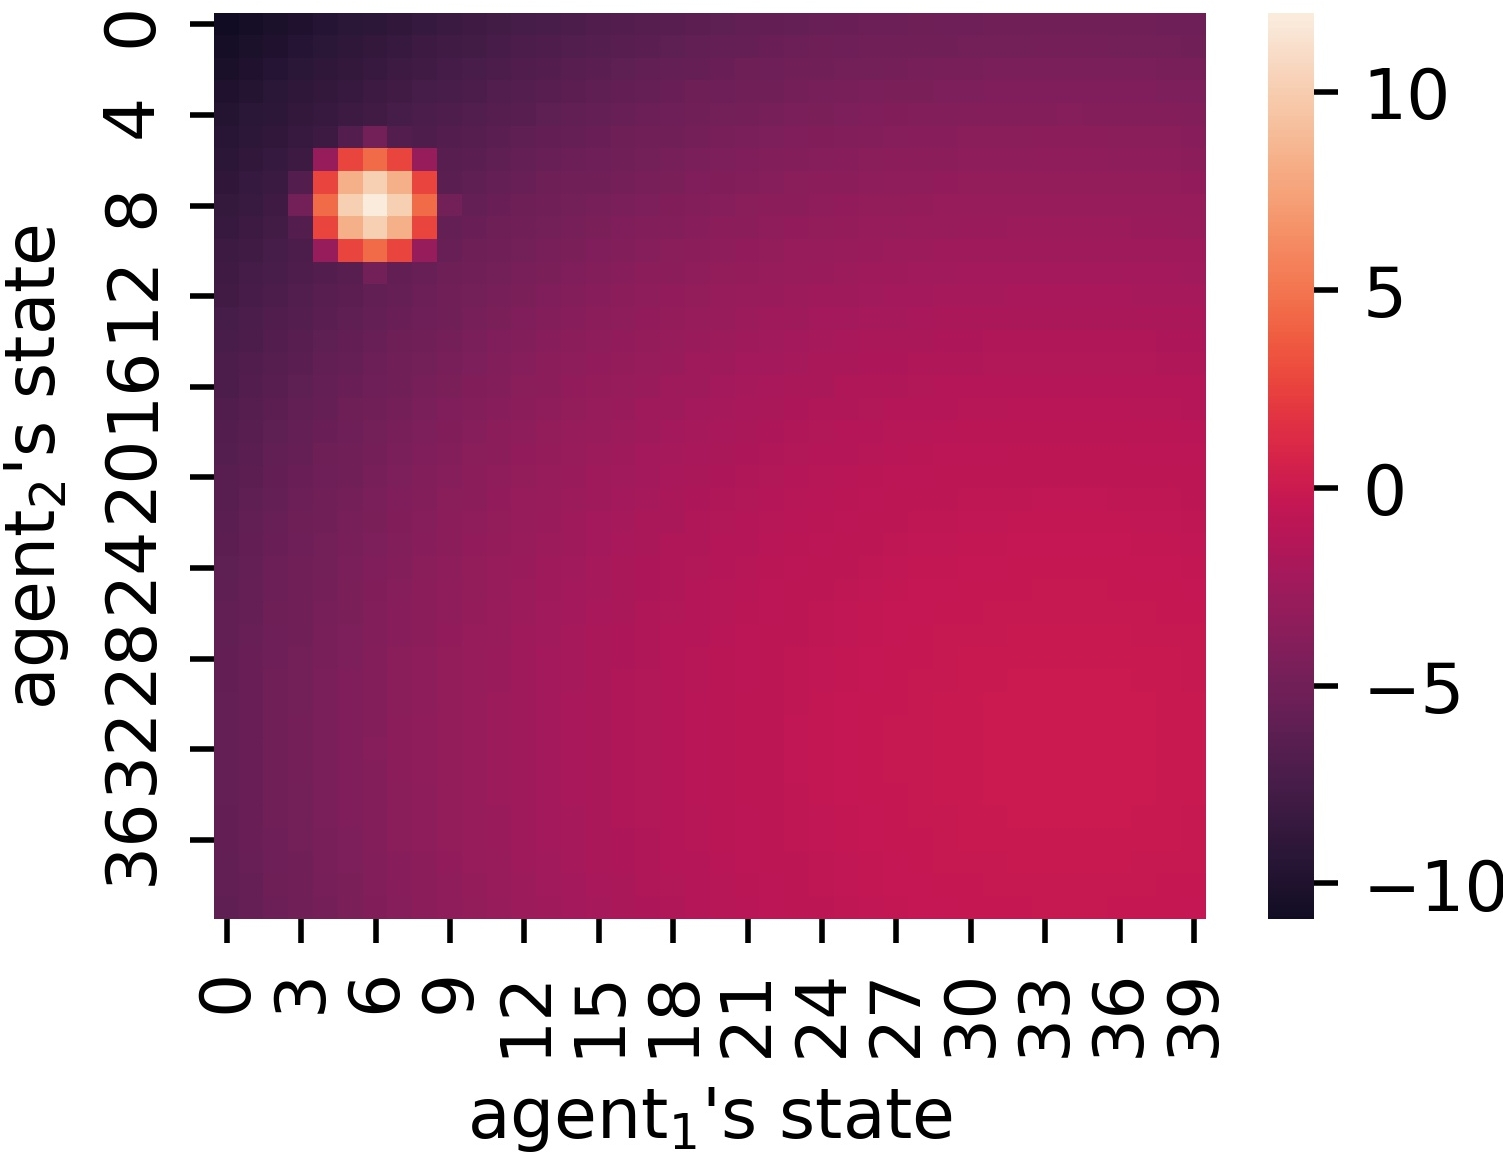
\includegraphics[width=0.5\linewidth]{Figures/JIM/ro_map30.jpg}
    \caption{Heat map of the rewards given for each state in the two-dimensional climbing game. Each axis show the positions of one agent. The combined position of the two agents yields a reward that is defined by Equation~\ref{eq:JIM:Climbing}. We distinguish clearly the high reward spike in the top-left of the environment and the low reward plateau in the bottom-right. The optimal strategy is to navigate towards the joint position corresponding to the high reward spike.}
    \label{fig:JIM:ro_map}
\end{figure}

To demonstrate how joint exploration helps solve the problem of relative overgeneralisation, we design a simple test environment that expands the example shown in Figure \ref{fig:JIM:ro_matrix}. This environment is a two-dimensional climbing game, inspired by previous works~\citep{Wei2018_MultiSoftQ}. In this environment, two agents can move on a discrete one-dimensional axis with $D$ possible positions. The two agents are denoted by their position, namely $\mathrm{x}$ (for the first agent) and $\mathrm{y}$ (for the second agent). At each time step, agents observe their position as a one-hot vector (e.g., for agent x, $o^\mathrm{x}_t=\{o^{\mathrm{x},i}_t=1\ \text{if}\ \mathrm{x}=i,\ 0\ \text{otherwise}\}_{0\leq i<D}$) and can choose between three actions: move in one direction or the other, or stay in position. They receive a reward corresponding to their combined position:
\begin{align}\label{eq:JIM:Climbing}
    \begin{split}
        r^{\text{ext}}_t(x,y;\delta)=\mathrm{max}\Bigl(&R^+-\frac{\delta}{D}\bigl[(x-r^+_x)^2+(y-r^+_y)^2\bigr],\\
        &R^--\frac{1}{8D}\bigl[(x-r^-_x)^2+(y-r^-_y)^2\bigr]\Bigr).
    \end{split}
\end{align}
The result of this formula is displayed in Figure \ref{fig:JIM:ro_map}. The reward combines two hyperboles in opposite corners: one narrow that culminates at $R^+$ at position $(r^+_x,r^+_y)$, and another much wider that plateaus at $R^-$ at position $(r^-_x,r^-_y)$. We set the optimal reward $R^+=12$ and the suboptimal $R^-=0$. The width of the optimal reward spike is controlled by the parameter $\delta$: a higher $\delta$ value yields a narrower spike. 

At the beginning of each episode, the agents are placed randomly on their respective axes. Each episode lasts $D$ steps, ensuring that all starting positions can reach all other positions on the axis. The goal of the agents is to find where to go to maximise the global return. The wide suboptimal hyperbole is deceptive as it is an obvious path for agents to minimise their loss. The optimal reward spike is difficult to find because it covers a small portion of the state space and is surrounded by very low rewards, but it guarantees much greater returns. We can vary the difficulty of the task by changing the width of this optimal reward spike: the narrower the spike, the harder it is to find. 

In this environment, we expect MADRL methods to struggle to find the optimal reward spike. Exploring local states could help but would not be sufficient to consistently solve the task. As the dimension $D$ of the local-state space is fairly small, local novelty rewards will quickly vanish and will not help agents find the optimal reward spike. Exploring the joint-observation space adequately is required in order to consistently find optimal rewards. As JIM will reward exploration until all combined positions $(x,y)$ are visited several times, agents will visit the optimal reward spike more often, thus helping them to learn the optimal coordinated strategy. 

\subsubsection{Results}

\begin{figure}
     \centering
     \begin{subfigure}[c]{\textwidth}
        \centering
        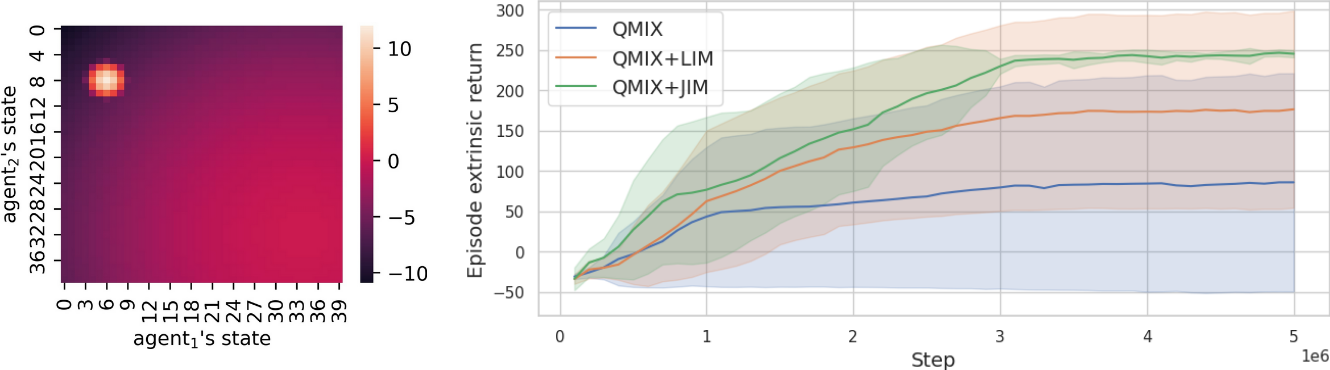
\includegraphics[width=\textwidth]{Figures/JIM/roR30.png}
        \caption{$\delta=30$}
        \label{fig:JIM:ro30}
     \end{subfigure}
     \vspace{1em}
     \begin{subfigure}[c]{\textwidth}
        \centering
        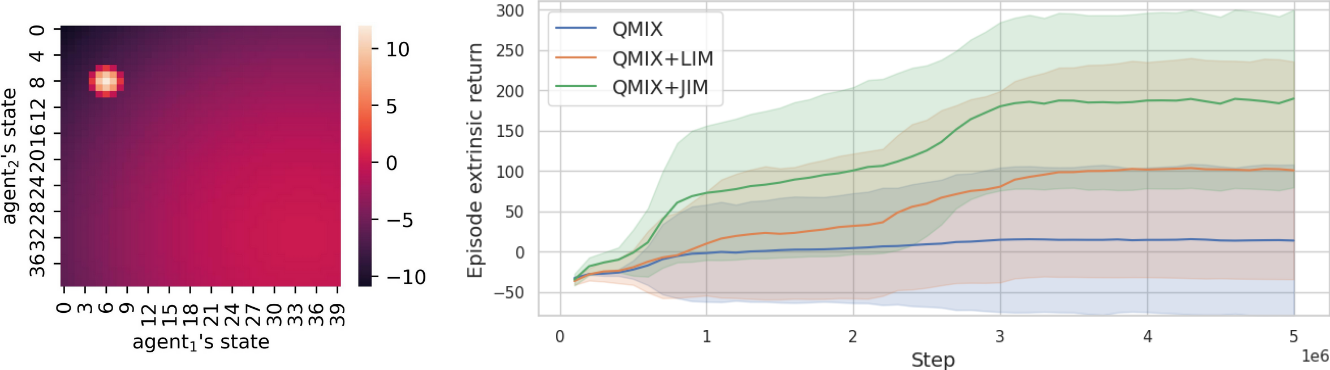
\includegraphics[width=\textwidth]{Figures/JIM/roR40.png}
        \caption{$\delta=40$}
        \label{fig:JIM:ro40}
     \end{subfigure}
     \vspace{1em}
     \begin{subfigure}[c]{\textwidth}
        \centering
        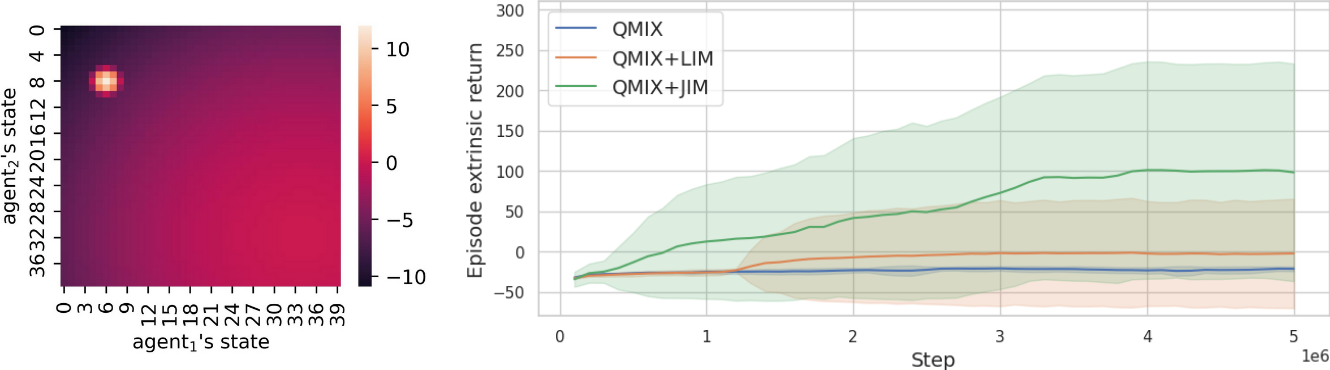
\includegraphics[width=\textwidth]{Figures/JIM/roR50.png}
        \caption{$\delta=50$}
        \label{fig:JIM:ro50}
     \end{subfigure}
     \caption{Performance of variants of QMIX in the climbing game, with three levels of difficulty. Each row corresponds to a different difficulty level, where difficulty is controlled by the width coefficient of the optimal reward spike $\delta$ (as defined in Eq. \eqref{eq:JIM:Climbing}). On the left are the heat maps representing the reward function in each instance. Increasing $\delta$ leads to a smaller optimal reward spike, thus making the task more difficult. On the right is shown the performance during training of QMIX with no intrinsic reward (QMIX), local intrinsic motivation (QMIX+LIM), and joint intrinsic motivation (QMIX+JIM) (mean and standard deviation shown for 15 runs each). We see that a slight decrease in the size of the optimal reward spike results in a considerable increase in the difficulty of the task.}
     \label{fig:JIM:ro_results}
\end{figure}

The results shown in Figure \ref{fig:JIM:ro_results} confirm the hypotheses formulated in the previous section. We show the performance of QMIX, QMIX+LIM, and QMIX+JIM across 15 independent runs each. Further, we present results in three difficulty levels dictated by the width of the optimal reward spike. The results clearly demonstrate the importance of exploring the joint-state space. QMIX alone manages to get a positive reward on the easy scenario, but its performance is lower and with a larger standard deviation compared to the two other algorithms, showing that some runs did not manage to find the optimal strategy. In the harder scenarios, QMIX's performance degrades strongly, never finding any positive reward in the hardest case. JIM clearly improves the performance of QMIX. In the easy scenario, QMIX+JIM consistently goes for the optimal reward spike. In the harder settings, it still performs well on average, even in the "very hard" scenario where the optimal reward spike covers only 0.013\% of all combined positions. The results of QMIX+LIM show that exploring the local-observation space helps agents find the optimal reward spike more often. However, it performs worse than JIM as it does not ensure that all combined positions are sufficiently explored. This shows that exploring the joint-observation space is crucial to allow agents to discover optimal coordinated behaviours.





\subsection{Coordination Task in a Continuous Environment}

\begin{figure}[h]
    \centering
    \setlength{\fboxsep}{0pt}
    \setlength{\fboxrule}{1pt}
    \fbox{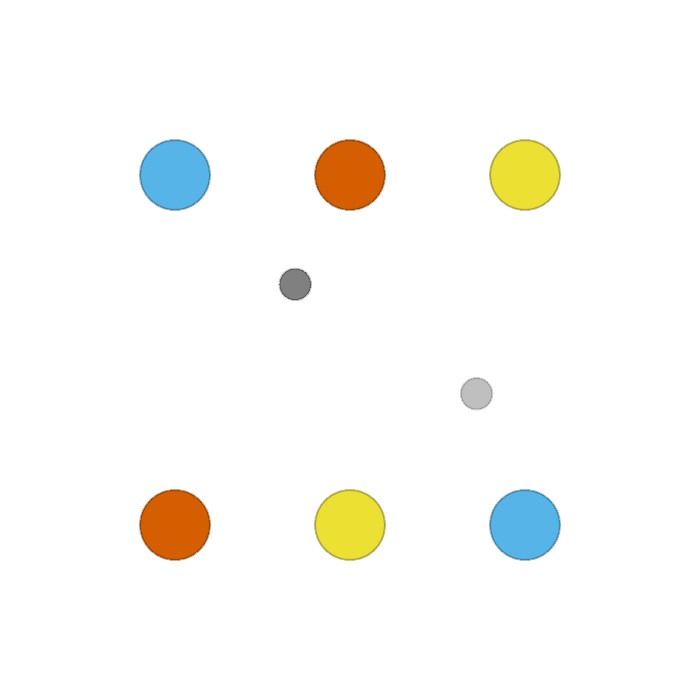
\includegraphics[width=0.4\textwidth]{Figures/JIM/push_buttons.jpg}}
    \caption{Coordinated placement task, agents are the small grey circles, the coloured circles represent landmarks the agents have to navigate on to gain rewards.}
    \label{fig:JIM:coord_place}
\end{figure}

\subsubsection{Environment Definition}

Next, we study how JIM scales to more realistic continuous environments and more complex tasks. We use the multi-agent particle environment (MPE;~\cite{Lowe2017_MADDPG}) to simulate a cooperative robotic task that requires a high degree of coordination. The state space of MPE is continuous: agents receive as observation a vector with their position in the two-dimensional space and relative positions and velocities of other entities. Agents navigate in a closed two-by-two-meter area by choosing between five discrete actions: move in any four cardinal directions or stay in place. The observation range is limited: agents only have information about entities that are in a range of 60 centimetres around them. 

We design a coordination task, named "\textit{coordinated placement}", where agents must position themselves over landmarks in order to maximise their returns. As shown in Figure \ref{fig:JIM:coord_place}, there are two sets of three coloured landmarks. The reward given at each time step depends on the placement of agents on the landmarks. The optimal state is having both agents placed on the orange landmarks, yielding a reward of +10 at each time step. The blue and yellow landmarks act as deceiving rewards, yielding much smaller rewards (+2 for blue, +1 for yellow). To increase the deceiving aspect of the blue and yellow landmarks, we also reward agents collectively by +0.5 if only one of them stands on one of these two colours. This leads to a relative overgeneralisation situation, as they will locally find that going on blue or yellow landmarks systematically leads to a reward, while this is not the case for orange. Only if agents explore their environment in a coordinated fashion, will they discover that they need to be both on orange to get the optimal reward signal. Importantly, this scenario features partial observability, with agents only having information about entities close to them. This means that agents do not necessarily see which landmark the other agent goes to. 

In this task, the observations of each agent consist in:
\begin{itemize}
    \item its personal information: its position and velocity $\mathtt{pos}_{\mathtt{self},x}$, $\mathtt{pos}_{\mathtt{self},y}$, $\mathtt{vel}_{\mathtt{self},x}$, $\mathtt{vel}_{\mathtt{self},y}$,
    \item information about the other agent: a boolean indicating if the other agent is visible or not, the relative position, and the velocity of this agent $\mathtt{is\_visible}_{\mathtt{agent}}$, $\mathtt{dist}_{\mathtt{agent},x}$, $\mathtt{dist}_{\mathtt{agent},y}$, $\mathtt{vel}_{\mathtt{agent},x}$, $\mathtt{vel}_{\mathtt{agent},y}$,
    \item for each landmark in the environment: a boolean indicating if the landmark is visible or not, the relative position of this landmark, and its colour as a one-hot encoding: $\mathtt{is\_visible}_{\mathtt{landmark}}$, $\mathtt{dist}_{\mathtt{landmark},x}$, $\mathtt{dist}_{\mathtt{landmark},y}$, $\mathtt{is\_red}$, $\mathtt{is\_blue}$, $\mathtt{is\_yellow}$.
\end{itemize}
Thus, the observation is a vector of dimension 43 containing this information. Relative positions of other entities (agent or landmarks) are actually the distance to the agent, normalised by their range of observation, i.e., 
$$\mathtt{dist}_{\mathtt{agent},x}=\frac{\mathtt{pos}_{\mathtt{agent},x}-\mathtt{pos}_{\mathtt{self},x}}{\mathtt{obs\_range}}.$$


\subsubsection{Results}

Experiments in the coordinated placement task demonstrate well the importance of exploring in a coordinated fashion. Figure~\ref{fig:JIM:coordplace_results} shows the performance across training of QMIX, QMIX+LIM, and QMIX+JIM, with 11 independent runs each. On the right is displayed the performance of each independent run at the last iteration of training. This helps to visualise the multiple modes in potential returns in this scenario. The coloured dashed lines give an insight into the level of strategy learnt by each run. These levels of strategy can be visualised with example trajectories displayed in Figure \ref{fig:JIM:coordplace_traj}. 

QMIX alone almost always goes for the blue landmarks, while sometimes settling for the yellow ones. This indicates that without actively exploring the environment, QMIX gets stuck because of deceptive rewards and is unable to find the optimal strategy. While QMIX+LIM seems slightly better than QMIX on the training curves, the individual run performance shows that LIM arguably performs worse. Two runs manage to find the optimal strategy, but LIM often performs poorly with only one agent on a blue or yellow landmark. This demonstrates that exploring the space of local observations can be helpful, as it pushes agents to explore the environment. However, it can also be misleading as they do not contain all the information about the current state of the environment. With JIM, exploring the joint-observation space clearly improves the quality of the chosen strategies. More than half of the time, QMIX+JIM finds the optimal reward signal and learns an effective strategy to go on orange landmarks, showing that JIM allows for more efficient exploration of coordinated behaviours. When agents do not find the optimal strategy, they stick with the best sub-optimal strategy to go both on blue. This shows that agents benefit from exploring the space of joint observations as they are directly linked to the obtained reward, whereas local observations lack crucial information to understand the global reward. 

The high standard deviation in the graph of Figure~\ref{fig:JIM:coordplace_results} is justified by the extreme gap in returns produced by the different levels of strategy. Note that this task is extremely sparse:
\begin{itemize}
    \item from a local perspective, because no guidance is given to agents to navigate towards any landmark;
    \item and from a joint perspective, as the optimal joint strategy is extremely marginal.
\end{itemize}
The deceptive rewards given by standing on blue or yellow make the suboptimal strategies very attractive. Without an explicit exploration strategy, QMIX is always attracted to the local optimum, similar to results found in the climbing game. Proper multi-agent exploration allows JIM to significantly improve the chances for QMIX to find the optimal strategy. 

\begin{figure}[t]
    \centering
    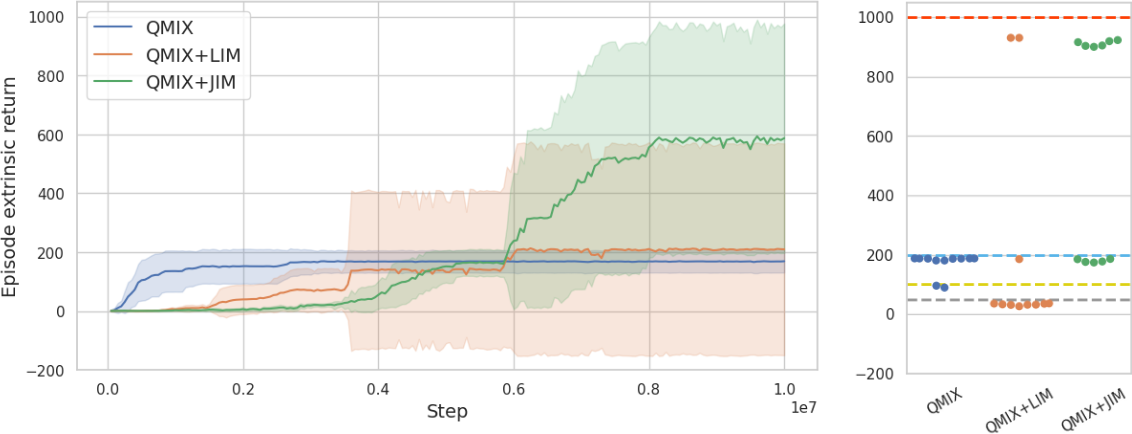
\includegraphics[width=0.95\textwidth]{Figures/JIM/coord_placeR.png}
    \caption{Performance of the three variants of QMIX in the coordinated placement task. The left shows the training curves with the mean and standard deviation across 11 independent runs each. The right graph displays the performance of each independent run at the last iteration of training. Dashed lines indicate the level of return obtained with different strategies: orange, blue, and yellow lines represent the return obtained if both agents are on landmarks of the related colour during 100 steps (the duration of an episode), and the grey line is for when only one agent is either on blue or yellow.}
    \label{fig:JIM:coordplace_results}
\end{figure}

\begin{figure}[t]
    \centering
    \centering
    \subcaptionbox{}{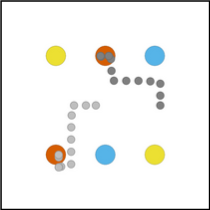
\includegraphics[width=0.22\textwidth]{Figures/JIM/traj1.png}}
    \subcaptionbox{}{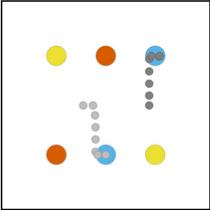
\includegraphics[width=0.22\textwidth]{Figures/JIM/traj2.png}}
    \subcaptionbox{}{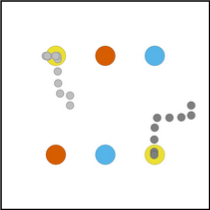
\includegraphics[width=0.22\textwidth]{Figures/JIM/traj3.png}}
    \subcaptionbox{}{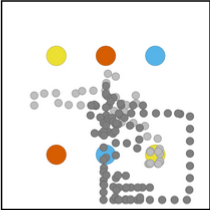
\includegraphics[width=0.22\textwidth]{Figures/JIM/traj4.png}}
    \caption{Examples of trajectories in the coordinated placement task. Each image displays a different level of strategy, with (a) > (b) > (c) > (d): (a) optimal strategy with both agents on orange, (b) both on blue, (c) both on yellow, and (d) one on blue/yellow.}
    \label{fig:JIM:coordplace_traj}
\end{figure}





\subsection{Further Analysis}

\subsubsection{Ablation Study}

Next, we propose an ablation study to compare JIM with two derived versions of the reward: one with only the \textit{episodic exploration criterion} $N_{EEC}$ (JIM-EEC) and one with only the \textit{life-long exploration criterion} $N_{LLEC}$ (JIM-LLEC). Note that JIM-LLEC is actually equivalent to NovelD \citep{Zhang2021_NovelD} in this environment as the episodic restriction of NovelD (see Section \ref{sec:JIM:IntrRew}) would be ineffective in a continuous environment such as MPE. 

\paragraph{Results} Figure \ref{fig:JIM:ablation_results} shows the results of training these versions in the coordinated placement task, with 11 independent runs each. Both ablated algorithms perform significantly worse than JIM. First, the episodic bonus of JIM-EEC alone lacks the motivation for discovering unseen configurations. Thus, it explores less and is not able to find the optimal solution to the task. Meanwhile, without the episodic restriction, JIM-LLEC is less driven to have diverse trajectories, hindering its exploration abilities. This confirms that, as shown in a recent study \citep{Andres2022_EvalIntrRew}, the episodic restriction implemented in NovelD and other intrinsic rewards \citep{Raileanu2020_RIDE,Badia2020_NGU} is crucial for developing efficient exploration strategies.  Overall, this proves the importance of combining the two stages of exploration defined in $N_{LLEC}$ and $N_{EEC}$. 

\begin{figure}[t]
    \centering
    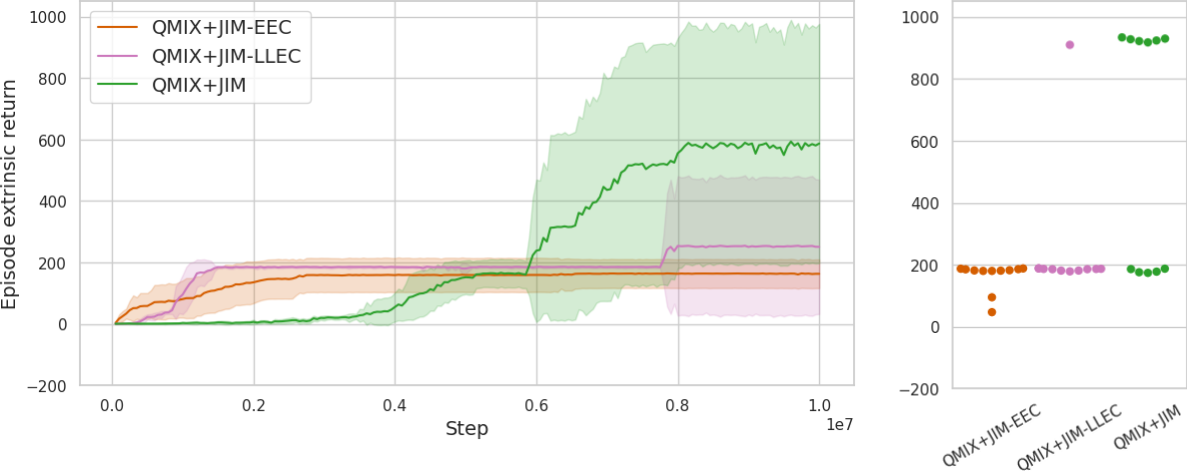
\includegraphics[width=0.95\textwidth]{Figures/JIM/ablationR.png}
    \caption{Ablation study of JIM in the coordinated placement task. The left graph shows the training curves with the mean and standard deviation across 11 independent runs each. The right graph displays the performance of each independent run at the last iteration of training. The two ablated versions only feature one of the two exploration criteria defined in Section \ref{sec:JIM:Algo}: JIM-EEC for $N_{EEC}$ and JIM-LLEC for $N_{LLEC}$. The results show the importance of combining the two criteria.}
    \label{fig:JIM:ablation_results}
\end{figure}




\subsubsection{Scaling Up to More Agents}\label{sec:JIM:Exp:scaling}

We evaluate JIM in a scenario with four agents using a modified version of the two-dimensional climbing game introduced in Section~\ref{sec:JIM:Exp_Climbing}. We modify the reward definition given Equation~\ref{eq:JIM:Climbing} to allow $N$ dimensions: 
$$
r^{\text{ext}}_t(\mathbf{p};\delta)=\mathrm{max}\left(R^+-\frac{\delta}{D}\sum_{i=0}^{N}(p_i-r^+_i)^2,R^--\frac{1}{8D}\sum_{i=0}^{N}(p_i-r^-_i)^2\right),
$$
with $\mathbf{p}=\{p_i\}_{0<i\leq N}$ the positions of the agents, $\delta$ the coefficient controlling the size of the optimal reward spike, $D$ the dimension of each agent's state, $R^+$ the maximum value of the optimal reward spike placed at position $\mathbf{r}^+=\{r^+_i\}_{0<i\leq N}$, and $R^-$ the maximum value of the suboptimal plateau placed at position $\mathbf{r}^-=\{r^-_i\}_{0<i\leq N}$. This formula yields the same results as the two-dimensional example shown in Figure~\ref{fig:JIM:ro_map} but in a $N$-dimensional space.

We use this extended version to experiment with a four-agent climbing game. As in the two-agent version, the reward function has a high reward spike in one corner of the space and a low reward plateau in the other corner, making relative overgeneralisation prone to arise. With more agents, the number of dimensions of the joint observation increases linearly (in this case: from 80 dimensions with two agents to 160 with four agents) while the number of possible states increases exponentially, making the search for the optimal strategy significantly more challenging.

To compensate for the increased size of the state space, we have to make the optimal reward spike larger for the task to be solvable by QMIX. In the four-agent experiments, we use $\delta=0.9$. 
Also, with four agents we had to lower the initial value of the $\epsilon$ parameter of QMIX for its $\epsilon$-greedy strategy. We found that increasing the number of agents led to bad results with the default $0.3$ initial value of $\epsilon$. With this hyperparameter set to $0.1$, the results were significantly better. This is likely due to the fact that agents choose separately if they explore or exploit, meaning that increasing the number of agents leads to more randomness in the selection of each joint action. 

\begin{figure}
    \centering
     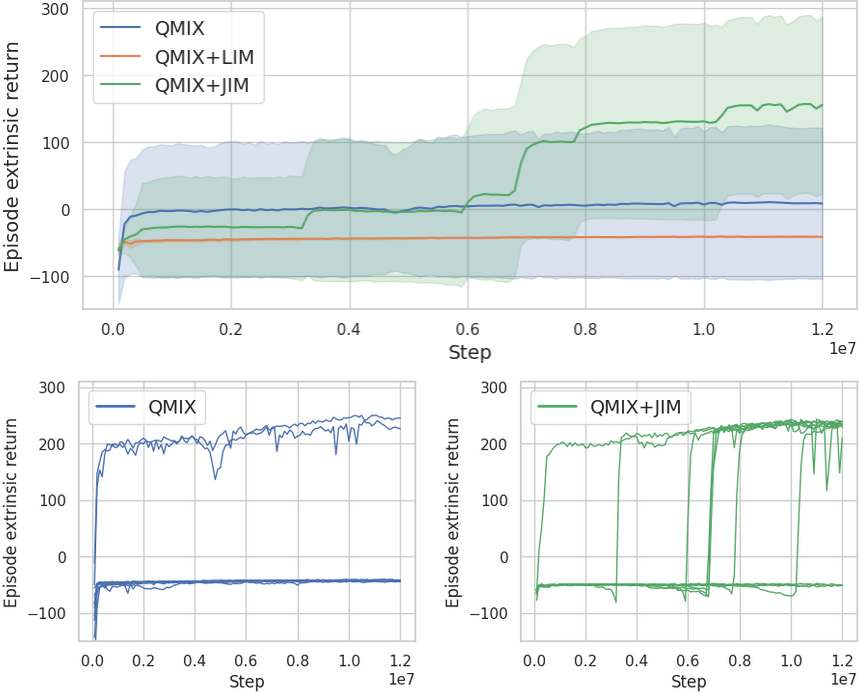
\includegraphics[width=0.8\textwidth]{Figures/JIM/climb4R.png}
    \caption{Training performance of QMIX, QMIX+LIM and QMIX+JIM in the four-agent climbing game. The top graph shows the mean and standard deviation across 11 runs each, the bottom graphs display all single runs for QMIX (left) and QMIX+JIM (right).}
    \label{fig:JIM:climb4_results}
\end{figure}

\paragraph{Results} Figure~\ref{fig:JIM:climb4_results} shows the results in this scenario for 11 independent runs each. As with previous experiments, JIM improves the performance of QMIX by upgrading its exploration capabilities. Taking a closer look at the results reveals that QMIX and QMIX+LIM find the optimal solution in respectively $2$ and $0$ runs out of the $11$, while QMIX+JIM finds the optimal solution in $8$ out of $11$ runs in the allocated time (see Figure~\ref{fig:JIM:climb4_results}-bottom).  
The two positive results for QMIX can be attributed to beneficial initial conditions as QMIX never reaches the optimal performance otherwise. This is not the case with QMIX+JIM, which shows robustness to initial conditions thanks to active exploration of the environment. In fact, the impact of JIM becomes evident when looking at curves from individual runs, where we consistently observe significant performance enhancements subsequent to a minor initial drop in efficiency. This phenomenon reflects a deliberate shift towards exploring novel approaches when the system would otherwise remain stagnant. This is unique to JIM, as  QMIX+LIM never succeeds in finding the optimal solution, advocating for the benefits of using a global, rather than local, intrinsic reward for exploration. 





\subsubsection{Cooperative Task with no Coordination Need}

\begin{figure}[h]
    \centering
    \setlength{\fboxsep}{0pt}
    \setlength{\fboxrule}{1pt}
    \fbox{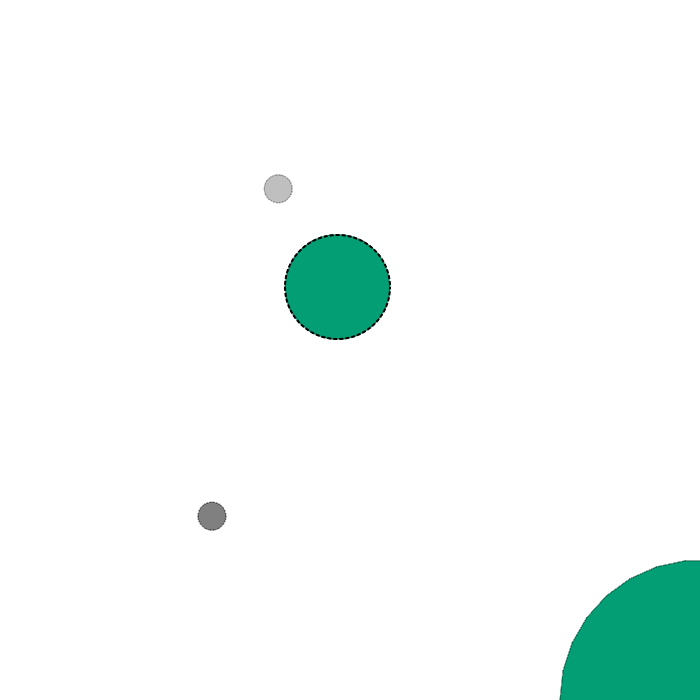
\includegraphics[width=0.4\textwidth]{Figures/JIM/coop_push.png}}
    \caption{Cooperative box pushing task, agents are the small grey circles, the green circle in the middle is an object to deliver to the landmark in the bottom right corner.}
    \label{fig:JIM:cooppush}
\end{figure}

To study coordinated exploration further, we experiment with a cooperative task that depends less on coordination. We design a cooperative box-pushing task that requires agents to push an object and place it on top of a landmark. Figure~\ref{fig:JIM:cooppush} shows a screenshot of this scenario. At the start of each episode, the landmark is randomly placed in any one of the four corners. The initial positions of the agents and the object are randomly set. If the agents manage to push the object and place it on the landmark, the episode ends early and they receive a reward of +100. Agents also get a small penalty of -1 at each time step to reward faster strategies. 

In this setting, observations are defined as:
\begin{itemize}
    \item its personal information: its position and velocity $\mathtt{pos}_{\mathtt{self},x}$, $\mathtt{pos}_{\mathtt{self},y}$, $\mathtt{vel}_{\mathtt{self},x}$, $\mathtt{vel}_{\mathtt{self},y}$,
    \item information about the other agent: a boolean indicating if the other agent is visible or not, the relative position, and the velocity of this agent $\mathtt{is\_visible}_{\mathtt{agent}}$, $\mathtt{dist}_{\mathtt{agent},x}$, $\mathtt{dist}_{\mathtt{agent},y}$, $\mathtt{vel}_{\mathtt{agent},x}$, $\mathtt{vel}_{\mathtt{agent},y}$,
    \item information about the object: a boolean indicating if the object is visible or not, the relative position, and the velocity of this object: $\mathtt{is\_visible}_{\mathtt{object}}$, $\mathtt{dist}_{\mathtt{object},x}$, $\mathtt{dist}_{\mathtt{object},y}$, $\mathtt{vel}_{\mathtt{object},x}$, $\mathtt{vel}_{\mathtt{object},y}$,
    \item and information about the landmark: a boolean indicating if the landmark is visible or not and the number of the corner it is located into (from 1 to 4): $\mathtt{is\_visible}_{\mathtt{landmark}}$, $\mathtt{corner}_{\mathtt{landmark}}$.
\end{itemize}
The observation is a vector of dimension 16 containing this information. Similarly to the coordinated placement task, this setting is also partially observable. 

\begin{figure}
    \centering
    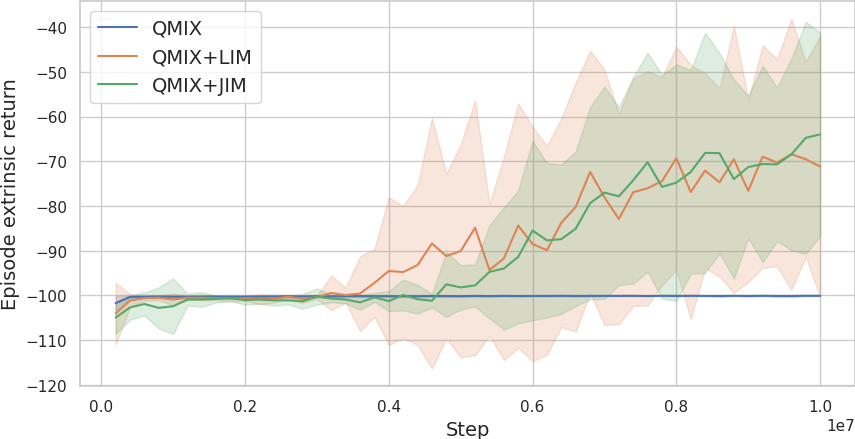
\includegraphics[width=0.8\linewidth]{Figures/JIM/cooppushR.png}
    \caption{Training curves of the three variants of QMIX in the cooperative box pushing task, with the mean and standard deviation across 11 runs each.}
    \label{fig:JIM:push_results}
\end{figure}

\paragraph{Results} Figure \ref{fig:JIM:push_results} shows the results in the cooperative push scenario (median and confidence interval shown for 11 runs each). First, we observe that QMIX alone performs very poorly as it is unable to find the solution to the task. The high sparsity of the reward function makes it impossible for agents to discover the objective with random exploration of the environment. Second, we see that JIM and LIM achieve similar levels of performance. While coordination can help agents perform well, it is actually not a requirement for this task. In fact, one agent alone is able to push the object and place it on the landmark. Thus, exploring the space of joint configurations is not helpful in this scenario. This shows however that actively exploring the environment is crucial in tasks where the reward function is very sparse. 




\subsubsection{Time Consumption}

\begin{figure}
    \centering
    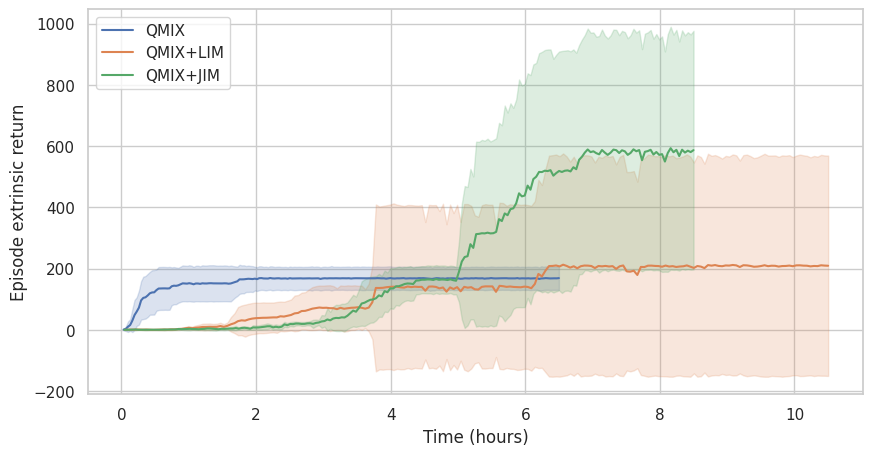
\includegraphics[width=0.8\textwidth]{Figures/JIM/time.png}
    \caption{Training curves of QMIX, QMIX+LIM, and QMIX+JIM in the coordinated placement task with execution time on the x-axis. In our implementation, using JIM increases training time by 31\%, and with LIM by 62\%.}
    \label{fig:JIM:time}
\end{figure}

Finally, we show another advantage of having a single, centralised intrinsic motivation. While LIM and similar approaches in previous works \citep{Iqbal2019_MultiExplore,Du2019_LIIR,Wang2020_EITI} require computing one intrinsic reward for each agent, JIM only computes one intrinsic reward for the whole group of agents. This makes JIM significantly more efficient to run, with LIM being approximately 24\% slower than JIM to train, as shown in Figure~\ref{fig:JIM:time}. 










% -------------------------------------------------------------------------------------------------

\section{Conclusion}

In this chapter, we present an algorithm for joint intrinsic motivation (JIM), which is the first method to reward active exploration of the joint-observation space. It can be integrated to enhance any MADRL algorithm that uses centralised training with decentralised execution. By combining JIM with the state-of-the-art QMIX algorithm, we demonstrate that it outperforms the original QMIX implementation, as well as a modified QMIX algorithm using local curiosity. We show that active exploration is a key component for multi-agent learning in environments with sparse rewards. Moreover, joint exploration enables the discovery of optimal coordinated behaviours that would be hard to find otherwise as they necessitate a high level of coordination between agents. 

This shows the importance of using joint observations in the process of computing intrinsic rewards for a multi-agent system. In fact, the joint observation is the best estimate of the global state of the environment available for the agents. Using it allows more efficient learning of multi-agent joint behaviours and is computationally less expensive than having to compute local intrinsic rewards for each agent. These results should encourage research on how joint observations can be used in other kinds of intrinsic rewards to shape the agents' behaviour further. 


